%!TEX root = report.tex

This model description follows the ODD format described by \textcite{grimm2006standard}. We start with a general overview of the agent-based model, followed by explanations of the design concepts, after which we discuss the details of the model. 

\begin{figure}
	\centering
	\begin{subfigure}{0.49\textwidth}
		\centering
		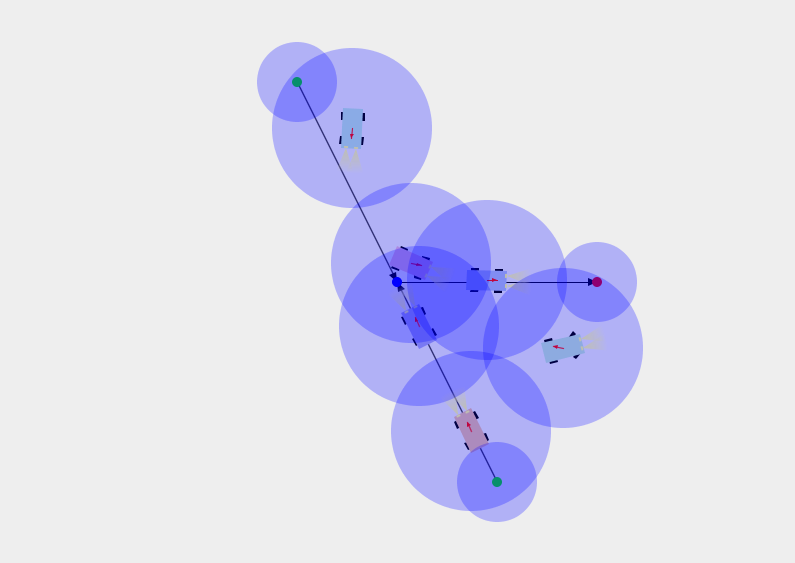
\includegraphics[width=\textwidth]{./img/simulationView1}
		\caption{With visible vision area.}
		\label{fig:model:simulation:fix}
	\end{subfigure}
	\begin{subfigure}{0.49\textwidth}
		\centering
		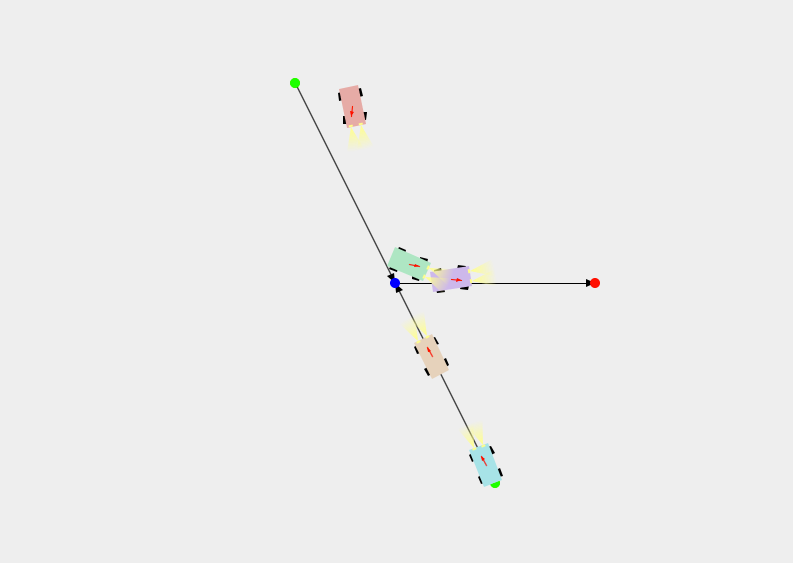
\includegraphics[width=\textwidth]{./img/simulationView2}
		\caption{Without visible vision area.}
		\label{fig:model:simulation:nofix}
	\end{subfigure}	
	\caption{The traffic simulation with \subref{fig:model:simulation:fix} visible vision area and \subref{fig:model:simulation:nofix} without visible vision area.}
	\label{fig:model:simulation}
\end{figure}

\subsubsection{Overview}
\label{subsub:method:model:overview}
%!TEX root = report.tex
\paragraph{Purpose}
\label{par:method:model:overview:purpose}
% \algemeen{A clear, concise and specific formulation of the model’s purpose. This element informs about why you need to build a complex model, and what, in general and in particular, you are going to do with your model.}

The purpose of this model is to have (build?) a traffic simulation in which we can test whether autonomous vehicles joining regular `human' traffic has an influence on the traffic delay experienced. To do this, we need a simulation in which we have different types of agents, the autonomous and the `human' ones, and a space that emulates a traffic simulation. In that simulation, we will let both types of agents drive over the roads, encounter intersections, and we will measure the delay an number of crashes. This we will do with different ratios of autonomous to human vehicles. 

\paragraph{State variables and scales}
\label{par:method:model:overview:state}

This model contains two different hierarchical levels, the Car/Driver level and the traffic level. The traffic level contains the possible roads and paths, and all the vehicles. The driver level contains all parameters necessary for the functioning of a vehicle.  

% The dimensions must be clearly defined for all parameters and variables in the tables.
	\subparagraph{Low-level state variables}
	The parameters described in \cref{tab:par:method:model:overview:state:lowlevel:car} are those contained by all drivers. 

	\later{Check that the low-level parameters are still accurate}

	\begin{table}[H]
		\centering
		\begin{tabular}{ >{\ttfamily}l  p{10.2cm} }
			\toprule
			\normalfont{Parameter}	& Purpose \\ 
			\midrule
			acceleration 			& Indicates if a vehicle has forward, backward, or no acceleration. \\ 
			targetBodyAngle 		& The angle at which the target is located, relative to the body of the vehicle. \\ 
			maxSteerAngleDeg 		& The maximum angle the wheels can turn. \\ 
			power 					& The impulse power of a vehicle. \\ 
			wheelAngleDeg 			& The current angle of the wheel, relative to the body of the vehicle. \\ 
			steeringSpeed 			& The speed with which a vehicle can turn (the turning radius). \\ 
			visionRange 			& The range of the vision of the vehicle. \\ 
			width 					& The width of the vehicle. \\ 
			length 					& The length of a vehicle. \\ 
			% colour 				& The colour of a vehicle \\ 
			driver 					& The driver agent. \\ 
			initialPosition 		& The initial position of the agent at the start of the simulation. \\ 
			% bodyFixture 			& The `fixture' of the bocy of a vehicle, used when viewing other vehicles\\ 
			% visionFixture 		& The `fixture of the vision of the vehicle, describing what a vehicle can see'\\ 
			targetSpeedKMH			& The maximum speed of a vehicle. \\ 
			path					& The path the agent is going to follow. \\ 
			\bottomrule
		\end{tabular}
		\caption{Car-owned state parameters}
		\label{tab:par:method:model:overview:state:lowlevel:car}
	\end{table}

	\subparagraph{Higher-level entities}
	
	\later{Check that the high-level parameters are still accurate}

	At the simulation level there are a few parameters, shown in \cref{tab:par:method:model:overview:state:highlevel:sim}. These are necessary for running the simulation.
	
	\begin{table}[H]
		\centering
		\begin{tabular}{ >{\ttfamily}l  p{10.5cm} }
			\toprule
			\normalfont{Parameter}	& Purpose \\  
			\midrule
			cars 					& A list of the cars in the simulation. \\ 
			streetGraph		 		& A graph representation of the network of streets. \\ 
			\bottomrule
		\end{tabular}
		\caption{Simulation-owned state parameters}
		\label{tab:par:method:model:overview:state:highlevel:sim}
	\end{table}


	\subparagraph{Scales}

	\later{Als er iets in tijdsstappen of planning verandert moet dit geupdate}

	Each time step is 33 ms. This was chosen because it is a frequent update rate that makes the visual of the simulation run smoothly, without creating a too large computational stress. Each step the agents get closer to their targets. The time horizon is longer, because each agent tries to follow a predetermined path. However, each agent also has to react to the environment. 



\paragraph{Process overview and scheduling}
\label{par:method:model:overview:process}
% \algemeen{Welke processen zitten in het model, eventueel met tabel.}

The processes active in the model are \t{steerToAvoidCars} and \t{steerTowardsPath}. 
The first checks if there is another vehicle in its vicinity and if it is going to hit it with the current driving angle. If so, the vector describing the direction the vehicle is going in is negated, causing the vehicle to decelerate or turn.
The second process is the driving of the vehicle in the direction of the target. The route towards this target has already been expressed in multiple points . A vehicle drives in the direction of the next point, and when it is close enough, drives to the one after that. Doing so, it will reach its goal, even when it gets diverted by other vehicles along the way.

% \algemeen{Bespreek scheduling van processen, welke volgorde uitgevoerd?}
Every step, each agent first checks if there are other cars it could possibly crash into before continuing on towards the target. 

% \algemeen{How is time modeled}
Time is modelled through the time steps in which a vehicle can move ahead. 

% \algemeen{How are actions that happen concurrently IRL executed in the model}
Actions that happen concurrently in real life are updating the position of every vehicle. In the simulation, this is done through choosing a small time step size, and updating every vehicle every time step. Because the time step is small enough, it will still approach a concurrent execution.

% \algemeen{Are some actions executed in a random order?}

There are no actions that are executed in a random order.


\subsubsection{Design Concepts}
\label{subsub:method:model:design}
%!TEX root = report.tex
% \algemeen{Bespreek (een subset van) de volgende elementen, niet noodzakelijk in deze volgorde.}

\later{Hiervoor moet het model meer af zijn.}

\paragraph{Emergence} 
% \algemeen{Which system-level phenomena truly emerge from individual traits, and which phenomena are merely imposed?}
There are no system-level phenomena that emerge from individual traits.

\paragraph{Adaptation} 
% \algemeen{What adaptive traits do the model individuals have which directly or indirectly can improve their potential fitness, in response to changes in themselves or their environment?}
The individuals have no adaptive traits.

\paragraph{Fitness} 
% \algemeen{Is fitness-seeking modelled explicitly or implicitly? If explicitly, how do individuals calculate fitness?}
Fitness-seeking is not modelled explicitly. 

\paragraph{Prediction} 
% \algemeen{In estimating future consequences of their decisions, how do individuals predict the future conditions they will experience?}
Agents are purely reactive, they do not not consider future conditions when deciding on their next action.  

\paragraph{Sensing} 
% \algemeen{What internal and environmental state variables are individuals assumed to sense or “know” and consider in their adaptive decisions?}
Individual vehicles can sense other vehicles and other objects if they are close enough to `see' them. They cannot see into each other's state variables, or those of the simulation. What is actual perceived by an agent depends on its type, self-driving versus human driver, and in the case of the human agent its state.

\paragraph{Interaction} 
% \algemeen{What kinds of interactions among individuals are assumed?}
Vehicles can observer other vehicles, but they cannot interact.

\paragraph{Stochasticity} 
% \algemeen{Is stochasticicity part of the model? What are the reasons?}
In this simulation everything is determined, there is no stochasticity.

\paragraph{Collectives} 
% \algemeen{Are individuals grouped into some kind of collective, e.g. a social group?}
There are no collectives in this simulation, all the agents function for themselves.

\paragraph{Observation} 
% \algemeen{How are data collected from the IBM for testing, understanding, and analysing it?}
The data we collect is with regard to the delay encountered while driving from one point to another, and the number of crashes. These measurements are discussed extensively in \cref{sub:method:design}.




\subsubsection{Details}
\label{subsub:method:model:details}
%!TEX root = report.tex 
\paragraph{Initialisation}
\label{par:method:model:details:initialization}
% \algemeen{How are the environment and the individuals created at the start of a simulation run, i.e. what are the initial values of the state variables? Is initialisation always the same, or was it varied among simulations? Were the initial values chosen arbitrarily or based on data? References to those data should be provided}
The initial variables are partly fixed, partly variable, an overview of all variables relating to cars and their initial values is presented in \cref{tab:par:method:model:details:init:car:value}. The variability is between agents, but not necessarily between simulations. These varying values are chosen arbitrarily for each run of the simulation.

\algemeen{Eenheden toevoegen aan \cref{tab:par:method:model:details:init:car:value}?}
\algemeen{En voor de random meuk even uitleggen hoe we ze bepalen, samled from a x distribution with mean blah.}
\begin{table}
	\centering
	\begin{tabularx}{\textwidth}{>{\ttfamily}lX}
		\toprule
		\normalfont{Parameter}	& Value \\  
		\midrule
		acceleration 			& NONE \\ 
		targetBodyAngle 		& 0 \\ 
		maxSteerAngleDeg 		& 40 \\ 
		power 					& 250 \\ 
		wheelAngleDeg 			& 0 \\ 
		steeringSpeed 			& 5 \\ 
		visionRange 			& 8 \\ 
		width 					& differs per vehicle \\ 
		length 					& differs per vehicle \\ 
		% colour 				& differs per driver type \\ 
		driver 					& a Driver object, determining the agent type \\ 
		initialPosition 		& differs per vehicle \\ 
		% bodyFixture 			& \\ 
		% visionFixture 		& \\ 
		targetSpeedKMH			& 0 \\ 
		path					& differs per vehicle \\ 
		\bottomrule
	\end{tabularx}
	\caption{An overview of the initialisation of car-owned state parameters.}
	\label{tab:par:method:model:details:init:car:value}
\end{table} 

\algemeen{Hebben we geen vaste init parameters voor de simulatie?}
The simulation variables differ per simulation, and so have no fixed initialisation settings.


\paragraph{Input}
\label{par:method:model:details:input}
% \algemeen{The dynamics of many IBMs are driven by some environmental conditions which change over space and time. All these environmental conditions are “input”, i.e. imposed dynamics of certain state variables.}

For this model the input is the graph of streets. The agents then get assigned a path to try to follow. 


% \paragraph{Submodels}
% \label{par:method:model:details:submodels}
%  No clue
